\documentclass[12pt,a4paper]{article}
\usepackage[utf8]{inputenc}
\usepackage{amsmath}
\usepackage{amsfonts}
\usepackage{amssymb}
\usepackage{minted}
\usepackage{graphicx}
\usepackage[linesnumbered,ruled,vlined]{algorithm2e}
\usepackage[margin = 2.00cm]{geometry}
\usepackage{tikz}
\usepackage{hyperref}
\hypersetup{
	colorlinks=true,
	linkcolor=black,
	filecolor=magenta,      
	urlcolor=black,
	pdfauthor=GHAOUI Mohamed Anis,
	pdfpagemode=Maximize,
	citecolor=black,
}


\author{GHAOUI M. Anis}
\title{Compte rendu TP A3 \\ Système électronique embarqué : Nios}
\date{25 - Mars - 2020}

\SetKwInput{KwInput}{Input}                % Set the Input
\SetKwInput{KwOutput}{Output}              % set the Output


%
\newcommand{\inputvhdl}[1]{\inputminted[linenos,tabsize=2]{vhdl}{./src/#1.vhd}}

\begin{document}
\maketitle
\hrule
\tableofcontents
\newpage

\section{Introduction}
La complexité de la conception des systèmes embarqués modernes étant devenue trop élevée, il est indispensable de recourir à des outils afin d'automatiser ce processus fastidieux. Dans le cours A3, on voit que les étapes de cette conception consistent en la préparation d'un système ayant un CPU virtuel dit \textit{SoftCore}, une ou plusieurs mémoire pour accompagner ce CPU et une brique FPGA qui agit comme un accélérateur matériel. 

Durant les séances de TP, on procède à la conception de plusieurs variante cette brique afin d'effectuer le calcul d'une racine carrée entière sur FPGA décrite en VHDL. Puis, on instancie un système embarqué grâce à l'outil Qsys d'Intel/Alter pour avoir un CPU et les périphériques requis. Enfin, on intégrera la brique conçue dans ce système afin de mesurer ses performances globales. 

Tous les codes et les projet Quartus peuvent être trouvés sur \href{https://github.com/anisghaoui/A3}{ce lien}.

\section{Conception d'opérateur racine carrée}
On commence par une analyse de l'algorithme afin de comprendre sa complexité et l'utilité d'accélérer un tel calcul matériellement.

\begin{algorithm}[H]
	\KwInput{(X,n) : X  entier codé sur $2\times n$ bits}
	\KwOutput{Z : Z entier codé sur n bits}
	Charger X
	
	$V = 2^{2n-2}$
	
	$Z=0$
	
	\For{i = n-1 à 0}{
		$Z =Z+V$
		
		\If{$X-Z\ge 0$}{
			$X=X-Z$
			
			$Z= Z+V$
		}
		\Else 
		{
			$Z=Z-V$
		}
		$Z=Z/2$
		
		$V=V/4$		
	}
	retourner Z
\end{algorithm}
%Q, ajoute des trucs

\subsection{Implémentation combinatoire}
Dans un premier temps, on pense à simplement traduire \textbf{tout} l'algorithme en vhdl dans un seul \textit{process} afin d'avoir une séquence d'éléments combinatoires propageant le résultat pour chaque valeur de i. Ceci sera synthétisé comme un circuit volumineux.
\paragraph{Résultats}
On voit sur la figure \ref{fig:oneprocess} le lancement du calcul sur le circuit combinatoire. celui ci est entre 2 coups d'horloges en simulation. Il sera contraint par les limites matérielles sur la carte. 
\begin{figure}[H]
	\centering
	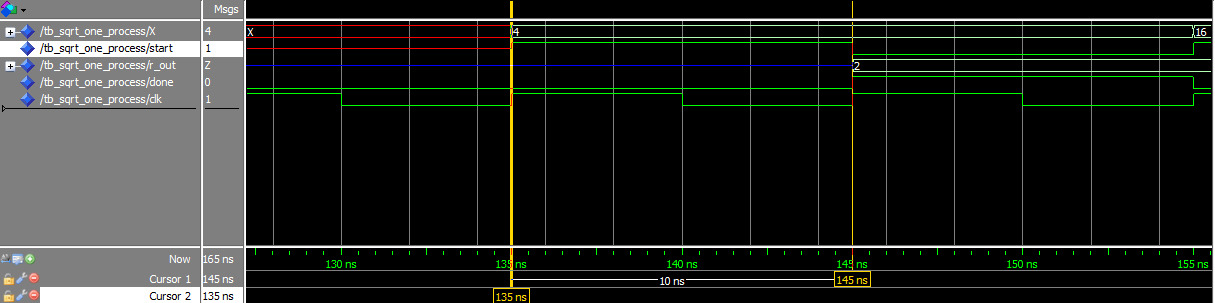
\includegraphics[width=\linewidth]{figures/one_process}
	\caption{Diagramme temporel du one process}
	\label{fig:oneprocess}
\end{figure}


\subsection{Implémentation multi-cycles}
\subsubsection{4 cycles}
On choisit alors d'implémenter une machine synchrone où on décrit le module de racine carrée par une machine d'états finis. il y aura un cycle où on itère $n$ fois . Le diagramme ci-dessous représente cet automate :
\begin{figure}[H]
\centering
\tikzstyle{nodus}=[circle,draw=black,minimum size=1.75 cm]
\def\dis{2}
\begin{tikzpicture}
\node [nodus] (wait)	[label={[label distance=0.5cm]90:!start}]  at (0,0) {wait};
\node [nodus] (init) 	[right of = wait,right = \dis cm] {init};
\node [nodus] (iter) 	[label={[label distance=0.5cm]-60:i!=n}]  [below of = init,below=\dis cm] {iter};
\node [nodus] (end) 	[below of = wait,below= \dis cm] {end};
\node [nodus] (default) [left of = wait,left = \dis cm] {default};

\draw [->] (wait) edge node [midway,above]{start}  (init);
\draw [->] (init)   edge (iter);
\draw [->] (iter)  edge node [midway,above]{i==n}  (end);
\draw [->] (end) edge (wait);
\draw [->] (default) edge (wait);

\draw [->](wait)  to[distance = 1 cm ,out=45,in=135] (wait);

\draw [->](iter)  to[distance = 1 cm ,out=-45,in=-90] (iter);

\end{tikzpicture}
\end{figure}

\paragraph{Résultats}
On voit sur la figure \ref{fig:5states} le lancement du calcul sur le circuit synchrone. On a alors une latence observable contrairement à celui en combinatoire.
\begin{figure}[H]
	\centering
	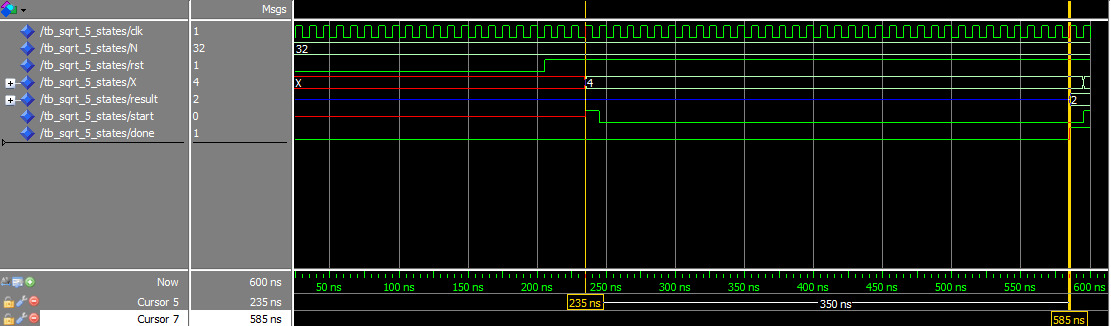
\includegraphics[width=\linewidth]{figures/5_stats}
	\caption{Diagramme temporel du 5 states}
	\label{fig:5states}
\end{figure}

\subsubsection{9 cycles}
Cette implémentation décompose relativement bien les états de l'automate. Mais, on pense pouvoir obtenir un gain de performances en ayant un cycle par opération à effectuer. L'idée est que vu que l'état sera combinatoirement simple, il sera plus rapide  à exécuter et donc la fréquence augmente. Par contre, on pense aussi que ceci consommera plus de ressources du FPGA.
\begin{figure}[H]
	\centering
	\tikzstyle{nodus}=[circle,draw=black,minimum size=1.5 cm,text width=1.5cm,align=center]
\def\dis{1.5}
\begin{tikzpicture}
\node [nodus] (wait)	[label={[label distance=0.5cm]90:!start}]  at (0,0) {wait};
\node [nodus] (init) 	[right of = wait,right = \dis cm] {init};
\node [nodus] (end) 	[below of = init,below= \dis cm] {end};
\node [nodus] (default) [below of = wait,below= \dis cm] {default};
\node [nodus] (iter1) [right of = init, right= \dis cm] {Rz+Rv};
\node [nodus] (iter2) [right of = iter1, right= \dis cm] {compare = Rx-Rz};

\node [nodus] (iter3_bis) [below of = iter2,below= \dis cm] {Rz-Rv};

\node [nodus] (iter3) [right of = iter2, right= \dis cm] {Rx-Rz};
\node [nodus] (iter4) [below of = iter3, below= \dis cm] {Rz+Rv};
\node [nodus] (iter5) [left of = iter3_bis, left= \dis cm] {Rz/=2 Rv/=2};


\draw [->] (wait) edge node [midway,above]{start}  (init);
\draw [->] (init)   edge (iter1);
\draw [->] (iter1) edge (iter2);
\draw [->] (iter2) edge node [rotate=60,midway,right]{$compare >= 0$}(iter3);
\draw [->] (iter3) edge  (iter4);
\draw [->] (iter4) to [in=-45,out=-135] (iter5);
%%%%%
\draw [->] (iter2) edge node [midway, right]{$compare < 0$}(iter3_bis);
\draw [->] (iter3_bis) edge (iter5);
%%%%%
\draw [->] (iter5) edge node [midway,below] {$i==1$}(end);
\draw [->] (iter5) edge node [midway,right] {$i > 1$} (iter1);

%\draw [->] (iter)  edge node [midway,above]{i==n}  (end);
\draw [->] (end) edge (wait);
\draw [->] (default) edge (wait);

\draw [->](wait)  to[distance = 1 cm ,out=45,in=135] (wait);


\end{tikzpicture}
\end{figure}


\paragraph{Résultats}
On voit sur la figure \ref{fig:9states} le lancement du calcul sur le circuit synchrone. On a plus de cycles de latence mais on pense que la fréquence de fonctionnement devrait être plus importante.
\begin{figure}[H]
	\centering
	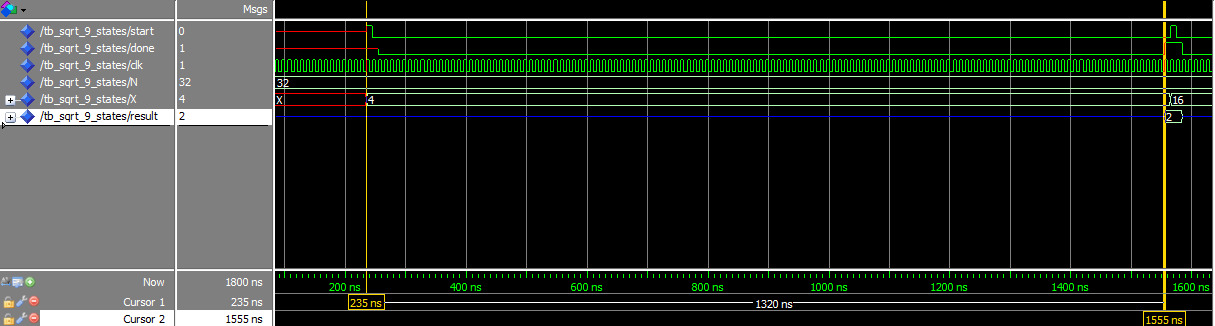
\includegraphics[width=\linewidth]{figures/9_stats}
	\caption{Diagramme temporel du 9 states}
	\label{fig:9states}
\end{figure}

\subsubsection{Variante "avare"} 
On procède a une variante dite "avare" qui va exploiter au mieux les mécanismes VHDL. Celle-ci parait offrir un compromis entre surface et fréquence.
\begin{figure}[H]
	\centering
	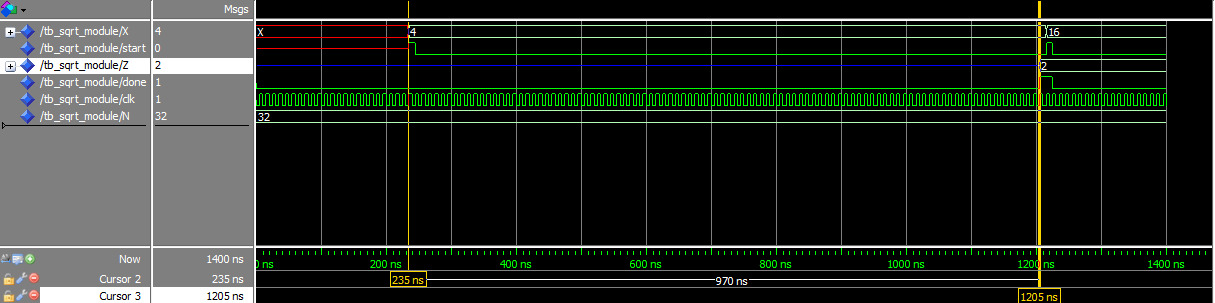
\includegraphics[width=\linewidth]{figures/sqrt}
	\caption{Diagramme temporel de sqrt}
	\label{fig:sqrt}
\end{figure}

%

\subsection{Implémentation avec opérateur unique}
On propose alors une implémentation avec un seul addition/soustracteur proposé dans l'énoncé. Ceci a pour but de diminuer le nombre d'éléments logiques utilisés. Il existe plusieurs implémentations de cet opérateur qui ont toutes comme contraintes de n'instancier qu'un seul opérateur qui est fourni par l'énoncé.

\subsubsection{Opérandes préemptées}
Dans cette variante, on positionne les variables à l'entrée de l'opérateur à un cycle avant leur utilisation. Ceci va contraindre la synthèse à avoir une période d'horloge plus grande que la durée de l'opération combinatoire d'addition/soustraction.
\begin{figure}[H]
	\centering
	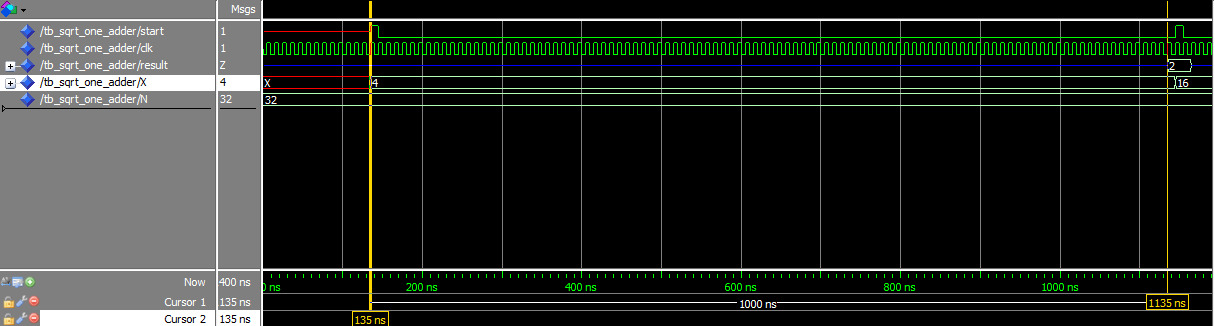
\includegraphics[width=\linewidth]{figures/one_adder}
	\caption{Diagramme temporel du one adder}
	\label{fig:one_adder}
\end{figure}
On constate sur la figure \ref{fig:one_adder} que le nombre de cycle est conséquent. On s'attend alors à ce que l'occupation matérielle soit moindre. On aura 2 versions de cette implémentation: l'une utilisant simplement un registre i pour compter, l'autre utilisant le décompteur fourni.
%

\subsubsection{Ségrégation des machines d'états} 
On procède à une séparation des machines d'états. On distingue la logique de contrôle synchrone de la logique de calcul qui est combinatoire. Ainsi, on aura plus de cycles mais beaucoup plus rapide et une consommation minime des ressources FPGA.
\begin{figure}[H]
	\centering
	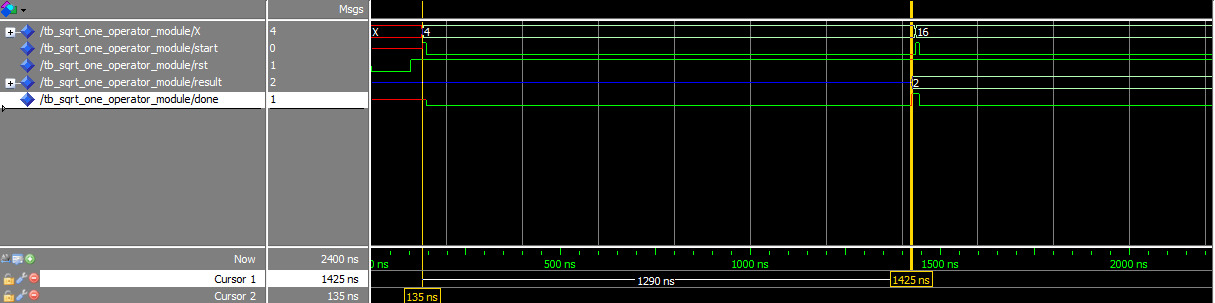
\includegraphics[width=\linewidth]{figures/one_operator}
	\caption{Diagramme temporel de one operator}
	\label{fig:one_operator}
\end{figure}


\subsection{Implémentation Pipeline}
Enfin, on pense à l'implémentation du module racine carrée en mode pipeline. On vise à ce que ce pipeline ait un intervalle d'initialisation de 1. i.e. qu'il puisse absorber une donnée à chaque nouveau cycle. Il aura naturellement une latence égale à n (nombre de bit de l'entrée) car chaque itération de la boucle d'algorithme est traité dans un étage.
\begin{figure}[H]
	\centering
	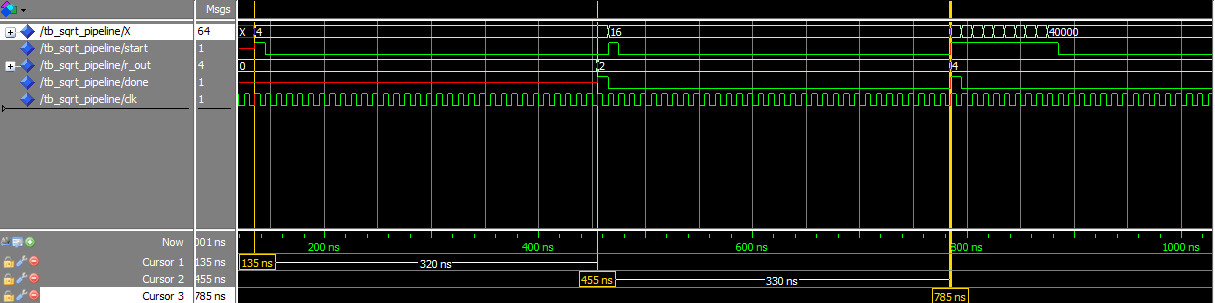
\includegraphics[width=\linewidth]{figures/pipeline}
	\caption{Diagramme temporel de pipeline}
	\label{fig:pipeline}
\end{figure}
La figure \ref{fig:pipeline} montre que le pipeline absorbe bien une donnée par cycle et que sa profondeur est de 32 cycles. Il important de noter qu'alimenter un tel pipeline ne sera pas évident car le Nios est incapable de charger/sauvegarder une donnée en 1 cycle. La mise est en place d'un DMA est envisageable mais ne sera vu dans ce rapport.


\section{Comparaison et résultat}
On remarque qu'il existe plusieurs compromis en termes de fréquences, surface FPGA. On peut par ailleurs comparer les différentes implémentations entre elles. On obtient ainsi les résultats suivants.
\begin{figure}[H]
	\centering
	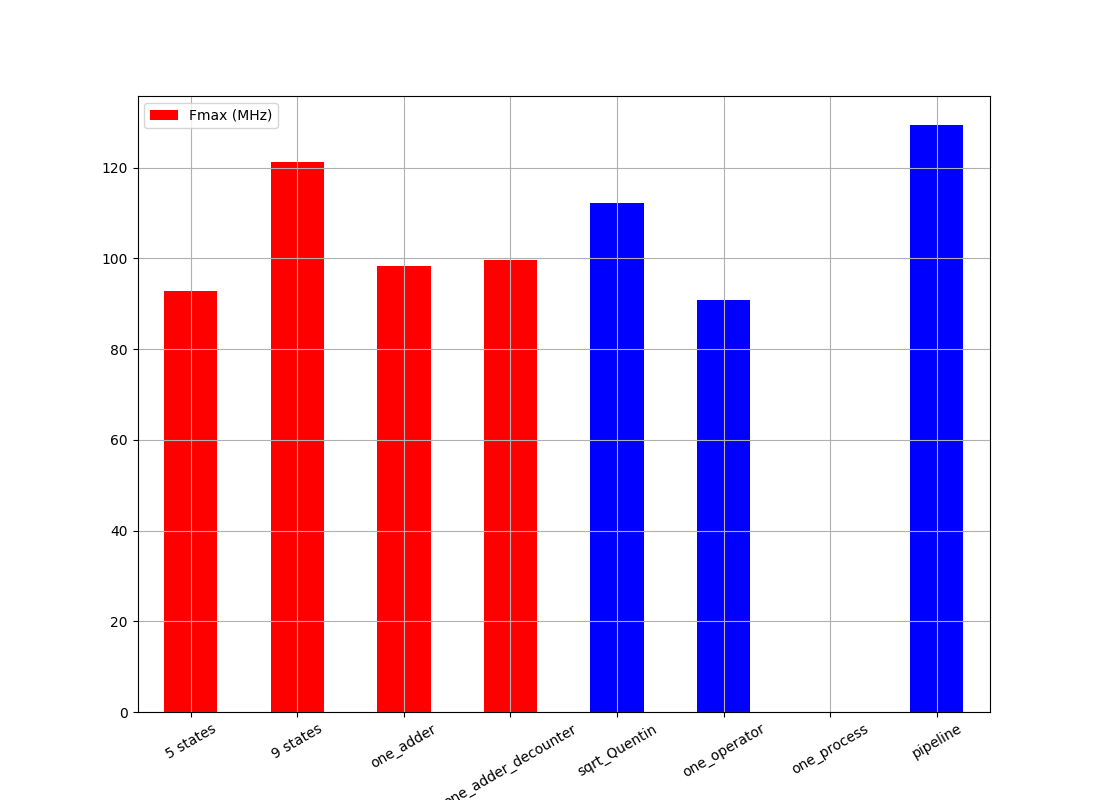
\includegraphics[width=0.7\linewidth]{mesures_freq/0}
	\caption{Mesures fréquentielles des différentes implémentations }
	\label{fig:0}
\end{figure}
On ne peut pas mesurer la fréquence de fonctionnement d'une circuit combinatoire sans imposer de registres à l'entrée et la sortie du circuit. On remarque que, comme attendu, on a un pipeline cadencé à une vitesse plus importante que les autres circuits. On remarque aussi que les circuits multi-cycles sont plus rapides que les circuits mono-opérateur. Ce qui est logique car elles prennent plus de place afin d'assurer une telle cadence.
\begin{figure}[H]
	\centering
	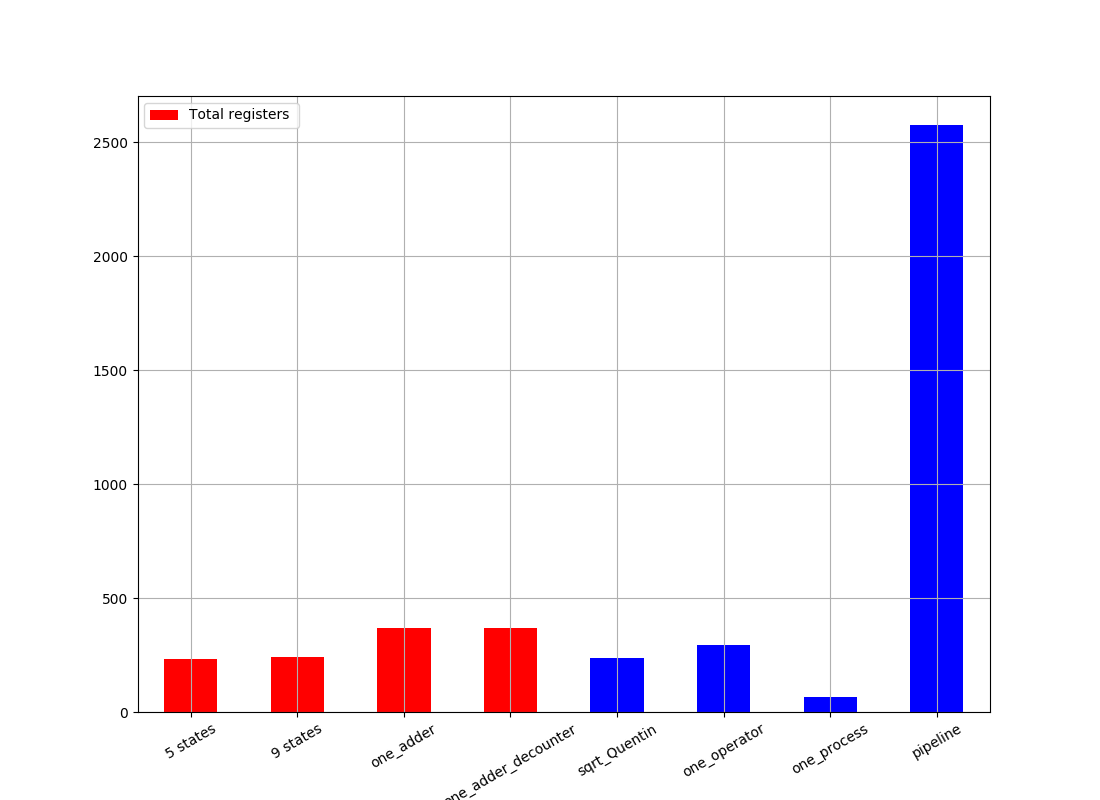
\includegraphics[width=0.7\linewidth]{mesures_freq/4}
	\caption{Usage de la surface FPGA par circuit implémenté}
	\label{fig:1}
\end{figure}
En terme de surface et éléments logiques occupés, la figure \ref{fig:1} montre que le pipeline occupé effectivement n fois plus de ressources car il y a bien n étages du même circuit. Aussi, on confirme bien les résultats trouvés en fréquentiel en observant que les mono-opérateurs sont plus économique en terme de surface FPGA.

\section{Conception du système embarqué} % 23-Jan
Le système embarqué sera implémenté sur une carte Intel/Altera Cyclone II De1. Au cœur de ce système : 
\begin{itemize}
\item un softcore le NIOS2 comme CPU
\item contrôleurs mémoires :
\subitem On-chip
\subitem SDRAM
\subitem SSRAM
\item périphérique JTAG permettant de programmer et déboguer le NIOS
\item module racine carrée VHDL
\end{itemize}
Par ailleurs, on utilisera des IP préconçues qui vont accélérer le développement du système. 


\subsection{Implémentation et programmation du Nios}
L'IP du softcore est fourni par Intel/Altera en plusieurs versions chacune offrant différentes cadences fréquentielles, caches instructions/données, opérateurs et pipeline. On ne détaillera pas ces différences ici car elles ont été vu en cours et peuvent être retrouvées dans la documentation d'Intel. On implémente donc les différentes versions telles que :
\begin{itemize}
\item Nios e : cache instructions 512 o
\item Nios s : cache instructions 512 o et données 512 o
\item Nios s : cache instructions 2 ko et données 2 ko
\item Nios f : cache instructions 512 o et données 512 o
\item Nios f : cache instructions 2 ko et données 2 ko
\end{itemize}
\subsection{Usage des différentes mémoires}
Grâce aux outils de développement proposés par Intel/Altera, on peut semi/automatiquement instancier de systèmes embarqués avec la possibilité de paramétrer l'emplacement mémoire du programme qui sera exécuté sur CPU. On peut alors écrire un programme qui calcule la racine carrée entière d'un nombre de manière logicielle, i.e. utiliser les opérateurs du NIOS. Ensuite, placer les données et le code dans soit la mémoire On-chip, SSRAM ou SDRAM. Ceci permet d'établir un comparatif entre ces différentes mémoires en termes de conception et timings pour plusieurs version du NIOS vues en cours. 

%Quentin ajoute ce que tu penses pértinant

\subsection{Comparaison des différentes implémentations}
On exécute le même programme C sur les différentes version du Nios. On mesure à chaque fois le temps d'exécution de ce code pour une mémoire et un version Nios.

\subsubsection{Mesure de temps}
Il existe plusieurs manières de mesurer le temps d'exécution sur Nios. Dans notre cas, on peut soit utiliser la bibliothèque fournie par le constructeur afin d'exploiter le registre compteur du Nios. Ou bien, implémenter nous-même ces fonctions de mesures afin d'avoir un plus grand contrôle sur la mesure de temps. Sans détailler, on opte pour implémenter ces fonctions et on les compare avec la version proposée par Altera :
$$
\begin{array}{cc}
	Impl\acute{e}mentation & \textit{temps de mesure à  vide ($\mu$)} \\ 
	Altera & 108 \\ 
	Personnalis\acute{e}e & 56 
\end{array} 
$$

On garde alors nos propres fonctions de mesures. On procède à une mesure fine du temps d'exécution. I.e. on  mesure le temps de lecture depuis un tableau, d'exécution de la fonction racine carrée et de l'écriture dans un tableau qui contient 1000 éléments.

\subsubsection{Temps mesurés}
On obtient alors le tableau suivant :
\begin{table}[H]
	\centering
		\ttfamily
	\begin{tabular}{|c|c|c|c|c|}	

		\hline
		Lecture ($\mu$s) & exécution ($\mu$s) & écriture ($\mu$s) & mémoire &  Nios  \\ \hline
		   951006    &     152117     &    143773     &  SDRAM  & 2k\_f  \\ \hline
		   920547    &     113891     &    107808     &  SSRAM  & 2k\_f  \\ \hline
		   864807    &     56543      &     52084     & ONCHIP  & 2k\_f  \\
		   \hline		  \hline
		  4408206    &     167321     &    174576     &  SDRAM  & 2k\_s  \\ \hline
		  1780954    &     86035      &     86012     &  SSRAM  & 2k\_s  \\ \hline
		  1332246    &     71018      &     71008     & ONCHIP  & 2k\_s  \\ 

		  \hline		  \hline

		  1021266    &     198997     &    142142     &  SDRAM  & 512\_f \\ \hline
		   946526    &     124316     &    102657     &  SSRAM  & 512\_f \\ \hline
		   911848    &     73247      &     57028     & ONCHIP  & 512\_f \\ 

		   \hline		  \hline

		  4407738    &     167296     &    174586     &  SDRAM  & 512\_s \\ \hline
		  1780954    &     86035      &     86012     &  SSRAM  & 512\_s \\ \hline
		  1332246    &     71018      &     71008     & ONCHIP  & 512\_s \\ 
		  \hline		  \hline

		  13484546    &     709816     &    713872     &  SDRAM  &   e    \\ \hline
		  5308056    &     316000     &    319000     &  SSRAM  &   e    \\ \hline
		  3992076    &     245000     &    248000     & ONCHIP  &   e    \\ \hline
	\end{tabular}
\rmfamily
\caption{Temps de lecture, d'exécution et écriture des différentes versions pour 1000 éléments}
\label{table:time}
\end{table}
On remarque que la version 2k\_f du Nios est la plus performante. Ceci est évident car c'est elle qui exploite le plus la surface du FPGA et possède des opérateurs en pipeline plus profonds. La mémoire Onchip est plus rapide que la SRAM et encore plus rapide que la DRAM du fait de la nature de conception des ces mémoires et la rapidité des accès. On remarque aussi qu'il y a des masquages des latences du chargement par la version 2k\_f.

En terme de surface FPGA, on peut voir sur le graphe suivant que la surface occupée est liée à la version du Nios. Plus la version est performante, plus elle occupera de la surface du FPGA.
\begin{figure}[H]
	\centering
	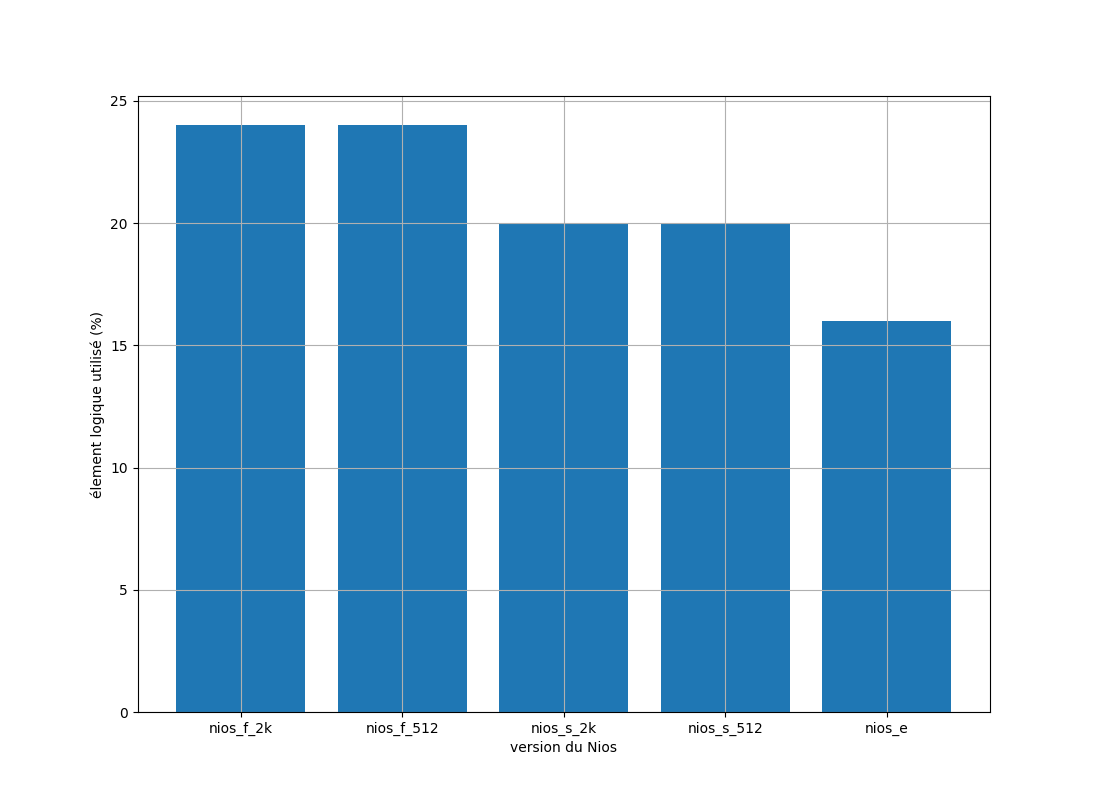
\includegraphics[width=0.8\linewidth]{figures/plot}
	\caption{Occupation des éléments logiques du FPGA}
\end{figure}
On voit ici l'occupation en termes d'éléments logiques. et que les mêmes versions de Nios occupent le même nombre d'éléments logiques mais un espace mémoire plus grand pour chacun des caches.

\subsection{Intégration du coprocesseur}
On veut instancier l'opérateur matériel afin d'accélérer le calcul. Dans un premier temps on génère par l'outil Qsys les entrées/sorties nécessaires pour communiquer avec l'opérateur matériel.

\subsubsection{Entrées/Sorties}
Les ports E/S peuvent être configurés en 4 modes : 
\begin{itemize}
	\item Entrée : Le Nios ne peut que lire cette adresse mémoire
	\item Sortie : Le Nios ne peut qu'écrire dans cette adresse mémoire
	\item Entrée/Sortie : Le Nios peut lire et écrire au choix
	\item E/S mixte : Le Nios peut lire et écrire au choix
\end{itemize}
Ces implémentations sont vues différemment au point de vu du VHDL. L'E/S mixte est un signal vu comme un \textit{inout}. Alors que le Entrée/Sortie
est vu en 2 signaux mais vu comme une seule variable coté C.

Au final, on a besoin des ports suivants :
\begin{itemize}
	\item Start/Done : 1 bit en entrée/sortie
	\item X  : 32 bits sortie
	\item Z : 32 bits entrée
\end{itemize}

Il suffit alors de créer une fonction qui positionne les variables puis lance les calculs en mettant \textit{Start} à 1 et attend (ou non) que \textit{Done} soit à 1. Le \textit{reset} est connecté au reset Nios. Une possible implémentation de la fonction est donnée ainsi :

\begin{minted}[linenos,numbersep=-5cm]{C}
			ushort sqrt_hw (uint X)
			{
				ushort z=0;
				*SQRT_X=X;
				*SQRT_status=1;
				while(0x1 & *SQRT_status != 1);
				*SQRT_status=0;
				z=*SQRT_result;
				return z;
			}
\end{minted}    

On peut choisir ou non d'enlever la ligne 7 afin d'avoir un code non-bloquant car le CPU est totalement libre durant tout le calcul.

\subsection{Intégration des instructions personnalisées}
On souhaite alors comparer ces implémentations avec une dernière qui va virtuellement augmenter l'ALU du Nios en ajoutant un des opérateurs racine carrée VHDL à ses opérateurs. Cette procédure consiste simplement à indiquer à l'outil Qsys quel circuit mettre comme opérateur ensuite le synthétiser afin d'avoir une macro-instruction qui agira comme une fonction. Un résultat possible de cette méthode : \mintinline{C}{ALT_CI_SQRT_MODULE_0(X)}

\subsection{Comparaison}
On compare les temps d'exécution des 2 implémentations précédentes au meilleur temps d'exécution (+lecture + écriture) du tableau \ref{table:time} pour la version \texttt{2k\_f}. On obtient les résultats suivants :
\begin{table}[H]
	\centering
	\ttfamily
	\begin{tabular}{c|c}
		Implémentation & Temps de mesuré ($\mu$s)  pour 1000 éléments\\ \hline  
		Logicielle & 973434\\
		Coprocesseur  & 297633\\
		Instruction personnalisée & 149633\\
	\end{tabular} 
\rmfamily
\caption{Comparatif entre les différentes implémentations}
\end{table}

On remarque que les implémentations matérielles sont beaucoup plus rapides que les implémentations logicielles. Ceci est naturel car c'est une des propriétés des conceptions en flot de données par rapport à une conception logicielle. On voit aussi que l'implémentation Coprocesseur est plus lente que l'instruction personnalisée car elle utilise de ports IO asynchrones pour communiquer avec le modules SQRT. On peut dire que l'instruction personnalisée est plus proche du CPU et donc plus rapide à interfacer. Par contre elle occupe le CPU pendant cet usage. Là où l'instruction personnalisée peut agir d'une manière non bloquante (type fire \& forget).

\newpage
\section{Conclusion}
Durant toutes ces séances de TP, on aura vu plusieurs aspects étudiés lors de ces dernières années. Que ce soit l'implémentation de brique VHDL ou les différents mécanismes dans une architectures CPU, les outils Intel/Altera facilement la mise en place de ces systèmes toujours plus compliqués.

Dans un premier temps, on a étudié et testé les différentes implémentations VHDL de l'algorithme racine carrée. On a pu les comparer en terme de latence et de surface FPGA. Dans un second temps, on a conçu un système électronique entièrement basé sur une carte FPGA. Ce système est facilement paramétrable d'un point de vu haut niveau même s'il repose sur plusieurs construction bas niveau qui nous sont abstraites. 

Par la suite, une fois le système implémenté, on a joué sur les différents curseurs à disposition pour pouvoir comparer l'exécution des différentes implémentations logicielles en utilisant les différentes mémoires et versions du Nios. On a pu voir l'effet des outils de mesures du temps sur ces performances.

Enfin on a comparé ces implémentations logicielles au implémentations hybrides utilisant une brique VHDL. Le constat est sans appel, les implémentations hybrides sont toujours plus rapides quelque soit l'interfaçage. Par manque de temps, on n'a pas pu implémenter l'usage du bus Avalon. Ceci n'aurait que confirmer ce résultat.



\end{document}